\chapter{Analysis of Parasite Clearance Times}
\section{Comparison of PC90 by experimental factors}
The derived PC90 values using the log-linear interpolation method are shown in Table \ref{derivedPC90}
\begin{table}[h]
\centering
\caption{Derived PC90 values in hours}\label{derivedPC90}
\begin{tabular}{|cc|c|c|}
\hline
&&\multicolumn{2}{c|}{Treatment}\\
&&alone&combined\\\hline
\multirow{2}{*}{Centre 1}&Male&$\begin{array}{c}3.85,\ 27.32,\ 36.30,\  8.84,\\4.35,\  1.53,\ 30.01,\  4.83\end{array}$&$\begin{array}{c}9.47,\  5.05,\  8.10,\\22.77,\  9.40,\  7.73\end{array}$\\\cline{2-4}
&Female&$\begin{array}{c}19.76,\ 22.45,\\21.75,\ 46.52\end{array}$&$\begin{array}{c}3.65,\ 8.40 ,\ 9.69,\\0.85,\ 9.04,\ 9.38\end{array}$\\\hline
\multirow{2}{*}{Centre 2}&Male&$\begin{array}{c}4.82,\ 2.21,\\11.59,\ 28.09\end{array}$&$\begin{array}{c}17.15,\ 9.51,\\14.68,\ 8.08\end{array}$\\\cline{2-4}
&Female&$\begin{array}{c}21.97,\ 2.49,\ 25.08,\ 31.63,\\5.00,\ 21.64,\ 24.42\end{array}$&$\begin{array}{c}14.77,\  8.75,\\5.84,\ 6.23\end{array}$\\\hline
\end{tabular}
\end{table}
\subsection{Graphical comparison}
The PC90 data from Table \ref{derivedPC90} are plotted by experimental factors centre, sex and treatment with 3 types of confidence intervals\footnote{The $t$ distribution and bootstrap confidence intervals are calculated using the \texttt{smean.cl.normal} and \texttt{smean.cl.boot} \emph{R} functions from the Hmisc library\cite{Hmisc}}:
\begin{description}
\item[Boxplots] - In Figure \ref{aov-box} the distribution of PC90 is summarized as boxplots, with the median, quartiles (the edges of the boxes) and 1.5 $\times$ the interquartile range (whiskers) shown.
\item[$t$ distribution] - In Figure \ref{aov-t} the mean is shown with 95\% confidence intervals from the $t$ distribution defined by the standard error of the data. These confidence intervals are relevant for normal parametric tests such as ANOVA and give an indication of differences that may be significant under such tests.
\item[Non-parametric] - In Figure \ref{aov-boot} the 95\% confidence intervals for the mean are derived from 1000 bootstrap samples of the data.
\end{description}
The observations we can make from Figures \ref{aov-box}, \ref{aov-t} and \ref{aov-boot} are as follows.
\begin{description}
\item[Treatment effect] - In the bottom-right panel of Figures \ref{aov-box} to \ref{aov-boot} the PC90 times for the 43 subjects are split into 23 and 20 alone (single) and combined drug treatment groups respectively. It can be seen that the subjects on the combined treatment appear to have clearance times, on average, around 10 hours shorter than those on the alone treatment. Subjects on the alone treatment show a larger spread of clearance times also. 
\item[Sex effect] - If we compare the bottom-left and bottom-centre panels in Figures \ref{aov-box} to \ref{aov-boot} 
\item[Centre effect] -
\item[Interactions] - 
\end{description}
\begin{figure}[h]
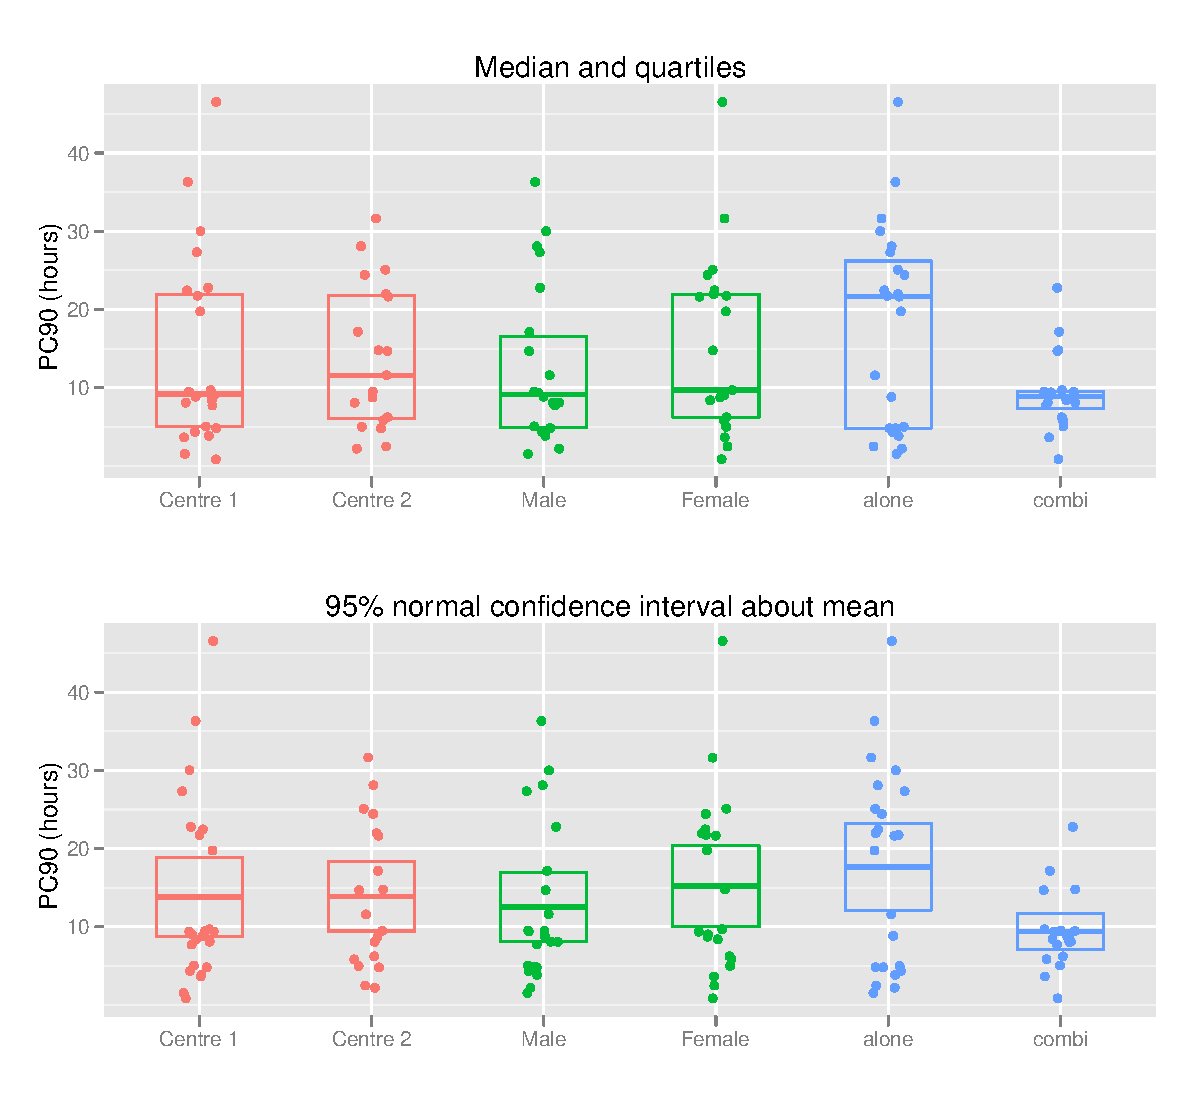
\includegraphics[width=6.5in]{pc90boxes.eps} 
\caption{Comparison of PC90 by experimental factors with boxplots showing the usual median, quartiles and 1.5 $\times$ IQR}
\label{aov-box}
\end{figure}
\begin{figure}[h]
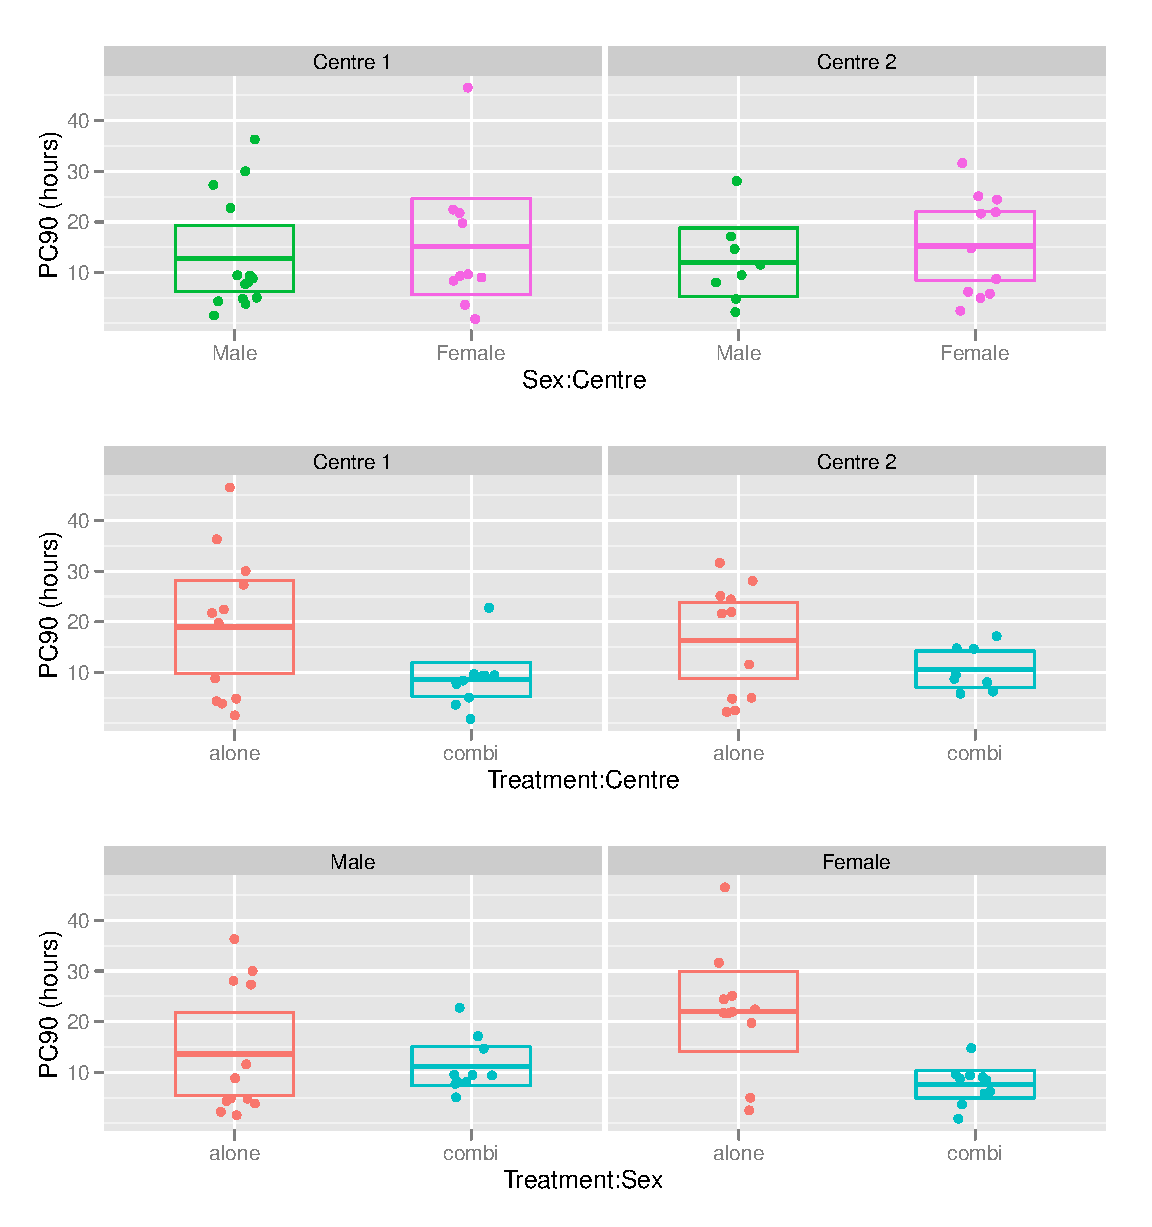
\includegraphics[width=6.5in]{pc90interaction.eps} 
\caption{Comparison of PC90 with 95\% confidence intervals from $t$ distribution defined by standard error of data}
\label{aov-t}
\end{figure}
3-way ANOVA with all interactions was performed on the PC90 data in Table \ref{derivedPC90}.

\subsection{ANCOVA}